\chapter{Rectangular Energy Estimates for the Dimensionless pTTM}
\label{app:ch2-rectangular-energy}

This appendix records a continuous energy estimate for the rectangular dimensionless pTTM used in Chapter~\ref{ch:numerical-methods}. The physical origin of the model is the axisymmetric pTTM of \eqref{eq:ch1-pttm}, together with the source construction of \eqref{eq:ch1-ulp_heat_source}. The analysis below is instead carried out for the rectangular computational problem \eqref{eq:ch2-dimensionless-pttm} on \(\Omega=[0,1]^d\), in the same geometry as the finite-difference schemes of Chapter~2.
The estimate concerns continuous PDE theory; it is not a discrete CN--CN or IMEX energy law.

\section{Rectangular spaces and coefficient-fixed weak formulation}
\label{sec:app-ch2-rectangular-spaces}

The coefficient-fixed problem is obtained on a positive temperature rectangle
\[
    \mathcal{R}\coloneqq [m_u,M_u]\times[m_v,M_v]\subset\mathbb{R}_{+}^{2},
\]
by replacing the nonlinear coefficients by bounded fixed quantities \(a_e,c_{1,*},c_{2,*}\) and by prescribed forcing \(s_*\). The coefficient \(a_e\) denotes the fixed divergence-form principal electron diffusion coefficient used in the weak problem below; it is not an exact Kirchhoff transformation of the full nonlinear pTTM.

\refstepcounter{theorem}
\paragraph{Remark \thetheorem\ (Admissible piecewise constitutive specifications).}\label{rem:app-ch2-piecewise-closures}
Piecewise polynomial or piecewise \(C^1\) closures for \(C_e\) and \(G\), such as the low-temperature and fitted regimes discussed in Chapter~1, are admissible examples for the coefficient assumptions used below. A typical schematic form is
\[
    C_e(u)
    =
    \begin{cases}
        \gamma u,                             & u<u_{\mathrm{cr}},    \\
        \displaystyle\sum_{k=0}^{P_e}a_k u^k, & u\ge u_{\mathrm{cr}},
    \end{cases}
    \qquad
    G(u)
    =
    \begin{cases}
        G_0,                                  & u<u_{\mathrm{cr}},    \\
        \displaystyle\sum_{k=0}^{P_G}b_k u^k, & u\ge u_{\mathrm{cr}},
    \end{cases}
\]
with the pieces chosen in \(\mathbb{R}[u]\). Imposing \(C^1\) matching at \(u_{\mathrm{cr}}\), for example equality of one-sided values and first derivatives, removes artificial jumps in the induced coefficients. On any compact temperature interval contained in \(\mathcal{R}\), these closures induce locally bounded coefficients \(D_1\), \(c_1\), and \(c_2\). If the pieces are matched continuously with bounded one-sided derivatives, and if \(C_e(T_{\mathrm{ref}}u)\) is bounded below by a positive constant on \([m_u,M_u]\), these induced coefficients are locally Lipschitz on the chosen rectangle. This remark is local in temperature and does not assert global regularity of the constitutive laws.

\subsection{Coefficient-fixed rectangular spaces and weak formulation}
\label{sec:app-ch2-frozen-weak-form}

Let \(\Omega=[0,1]^d\), with \(d\in\{1,2,3\}\), and let
\[
    H\coloneqq L^2(\Omega),
    \qquad
    (p,q)_H\coloneqq\int_{\Omega}p q\,d\mathbf{x},
    \qquad
    V\coloneqq H^1_0(\Omega).
\]
The space \(V\) corresponds to the homogeneous Dirichlet problem obtained after lifting any prescribed boundary data. Thus, in this appendix, \(u\) and \(v\) denote the homogeneous-trace unknowns after such a lifting. For a periodic Cauchy calculation, \(V\) may be replaced by the corresponding periodic \(H^1\) space; the estimates below use only the fact that boundary terms vanish. Define
\[
    \mathbb{H}\coloneqq H\times H,
    \qquad
    \mathbb{V}\coloneqq V\times V,
\]
with the natural product norms. Let \(a_e,c_{1,*},c_{2,*}\in L^{\infty}((0,\tau_f)\times\Omega)\) satisfy
\[
    0<\lambda_e\le a_e\le\Lambda_e,
    \qquad
    0\le c_{1,*},c_{2,*}\le C_c,
    \qquad
    D_2>0,
\]
almost everywhere, and let \(s_*\in L^2(0,\tau_f;V')\) be prescribed forcing. Here \(a_e\) denotes a fixed rectangular electron diffusion coefficient corresponding to the principal diffusion factor in Chapter~2, while \(c_{1,*}\) and \(c_{2,*}\) denote fixed coupling rates.

\refstepcounter{theorem}
\paragraph{Definition \thetheorem\ (Coefficient-fixed rectangular weak formulation).}\label{def:app-ch2-rectangular-weak-form}
A pair \((u,v)\) is a weak solution of the coefficient-fixed rectangular problem if
\[
    (u,v)\in L^2(0,\tau_f;\mathbb{V}),
    \qquad
    (\partial_tu,\partial_tv)\in L^2(0,\tau_f;\mathbb{V}'),
\]
and, for all \((\phi,\psi)\in\mathbb{V}\) and almost every \(t\in(0,\tau_f)\),
\begin{align}
    \langle\partial_tu,\phi\rangle_{V',V}
    +
    (a_e\nabla u,\nabla\phi)_H
    +
    (c_{1,*}(u-v),\phi)_H
     & =
    \langle s_*,\phi\rangle_{V',V},
    \label{eq:app-ch2-rectangular-weak-u}
    \\
    \langle\partial_tv,\psi\rangle_{V',V}
    +
    D_2(\nabla v,\nabla\psi)_H
    -
    (c_{2,*}(u-v),\psi)_H
     & =
    0.
    \label{eq:app-ch2-rectangular-weak-v}
\end{align}
The source is treated as prescribed in this appendix. Any solution dependence of \(s(t,\mathbf{x};u,v)\) in Chapter~2 must be handled separately as a nonlinear perturbation.

\begin{lemma}[Rectangular Green identity]
    \label{lem:app-ch2-rectangular-green}
    Let \(a\in W^{1,\infty}(\Omega)\) satisfy \(a\ge\lambda>0\). Let \(w\in H^2(\Omega)\cap V\) and \(\phi\in V\), or more generally assume \(a\nabla w\in H(\operatorname{div};\Omega)\), where
    \[
        H(\operatorname{div};\Omega) \coloneqq \{ \mathbf{v} \in L^2(\Omega; \mathbb{R}^d) \mid \nabla \cdot \mathbf{v} \in L^2(\Omega; \mathbb{R}) \}.
    \]
    If the boundary contribution vanishes by homogeneous Dirichlet, periodic, or compatible Cauchy data, then
    \[
        \int_{\Omega}\nabla\!\cdot(a\nabla w)\,\phi\,d\mathbf{x}
        =
        -
        (a\nabla w,\nabla\phi)_H.
    \]
\end{lemma}
\begin{proof}
    The test function is \(\phi\). Applying Green's formula, in the classical form recorded in \cite[Appendix~C.2]{Evans_2010}, to \(\nabla\!\cdot(a\nabla w)\phi\) gives
    \[
        \int_{\Omega}\nabla\!\cdot(a\nabla w)\phi\,d\mathbf{x}
        =
        \int_{\partial\Omega}\phi\,a\nabla w\cdot\mathbf{n}\,dS
        -
        \int_{\Omega}a\nabla w\cdot\nabla\phi\,d\mathbf{x}.
    \]
    This is the only integration-by-parts step. The boundary term vanishes because \(\phi=0\) on \(\partial\Omega\), or by cancellation over opposite faces in the periodic variant. The stated identity follows. The \(H(\operatorname{div};\Omega)\) formulation is obtained by the same identity in the weak normal-trace sense; see the same appendix for the density passage from smooth functions to Sobolev traces.
\end{proof}

\begin{lemma}[Diffusion coercivity and G{\aa}rding control]
    \label{lem:app-ch2-rectangular-diffusion-coercivity}
    Under the coefficient assumptions above, define
    \[
        \mathcal{A}_D((u,v),(\phi,\psi))
        \coloneqq
        (a_e\nabla u,\nabla\phi)_H
        +
        D_2(\nabla v,\nabla\psi)_H.
    \]
    Then there exist constants \(\alpha_D>0\) and \(\omega_D\ge0\), depending only on \(\lambda_e\), \(D_2\), and \(\Omega\), such that
    \[
        \mathcal{A}_D((u,v),(u,v))
        +
        \omega_D\|(u,v)\|_{\mathbb{H}}^2
        \ge
        \alpha_D\|(u,v)\|_{\mathbb{V}}^2
    \]
    for all \((u,v)\in\mathbb{V}\). This is the usual G{\aa}rding lower bound for uniformly elliptic bilinear forms; compare \cite[Section~6.2, Theorem~1]{Evans_2010}. For the homogeneous Dirichlet space \(V=H^1_0(\Omega)\), Poincar\'e's inequality \cite[Section~5.8.1, Theorem~1]{Evans_2010} allows the same estimate to be written with an equivalent gradient norm and no lower-order term.
\end{lemma}
\begin{proof}
    Use the test pair \((u,v)\). With
    \[
        \alpha_0\coloneqq\min\{\lambda_e,D_2\}>0,
    \]
    the coefficient lower bound gives
    \[
        \mathcal{A}_D((u,v),(u,v))
        =
        (a_e\nabla u,\nabla u)_H
        +
        D_2\|\nabla v\|_H^2
        \ge
        \alpha_0
        \left(
        \|\nabla u\|_H^2+\|\nabla v\|_H^2
        \right).
    \]
    Adding \(\omega_D\|(u,v)\|_{\mathbb{H}}^2\), for instance with \(\omega_D=\alpha_0\), yields the stated G{\aa}rding form after adjusting the constant \(\alpha_D\). If \(V=H^1_0(\Omega)\), Poincar\'e's inequality controls the \(H\)-part of the norm by the gradient part, so the lower-order term can be dropped when the equivalent gradient norm is used.
\end{proof}

\begin{lemma}[Control of the coefficient-fixed coupling form]
    \label{lem:app-ch2-rectangular-coupling-control}
    Under the coefficient assumptions above, define
    \[
        \mathcal{A}_C((u,v),(u,v))
        \coloneqq
        (c_{1,*}(u-v),u)_H
        -
        (c_{2,*}(u-v),v)_H.
    \]
    Then
    \[
        \left|\mathcal{A}_C((u,v),(u,v))\right|
        \le
        C_C\|(u,v)\|_{\mathbb{H}}^2,
    \]
    where \(C_C\) depends only on \(C_c\). If \(c_{1,*}\) and \(c_{2,*}\) are positive constants, testing the electron equation with \(c_{2,*}u\) and the lattice equation with \(c_{1,*}v\) gives the non-negative left-hand contribution
    \[
        c_{1,*}c_{2,*}\|u-v\|_H^2.
    \]
\end{lemma}
\begin{proof}
    The proof uses the test pair \((u,v)\). By Cauchy--Schwarz, Young's inequality, and \(0\le c_{1,*},c_{2,*}\le C_c\),
    \[
        |(c_{1,*}(u-v),u)_H|
        \le
        C_c\|u-v\|_H\|u\|_H
        \le
        C_c
        \left(
        \frac{3}{2}\|u\|_H^2+\frac{1}{2}\|v\|_H^2
        \right),
    \]
    and similarly
    \[
        |(c_{2,*}(u-v),v)_H|
        \le
        C_c
        \left(
        \frac{1}{2}\|u\|_H^2+\frac{3}{2}\|v\|_H^2
        \right).
    \]
    Therefore
    \[
        \left|\mathcal{A}_C((u,v),(u,v))\right|
        \le
        2C_c
        \left(
        \|u\|_H^2+\|v\|_H^2
        \right),
    \]
    which is the desired bound after renaming the constant. In the constant-coefficient case, direct expansion gives
    \[
        c_{2,*}c_{1,*}(u-v,u)_H
        -
        c_{1,*}c_{2,*}(u-v,v)_H
        =
        c_{1,*}c_{2,*}\|u-v\|_H^2.
    \]
\end{proof}

\begin{theorem}[A priori energy estimate for the coefficient-fixed rectangular problem]
    \label{thm:app-ch2-rectangular-energy}
    Let \((u,v)\) be a weak solution in the sense of Definition~\ref{def:app-ch2-rectangular-weak-form}, with initial trace \((u(0),v(0))=(u_0,v_0)\in\mathbb{H}\). Assume
    \[
        0<\lambda_e\le a_e\le\Lambda_e,
        \qquad
        0\le c_{1,*},c_{2,*}\le C_c,
        \qquad
        D_2>0,
        \qquad
        s_*\in L^2(0,\tau_f;V').
    \]
    Then there exists a constant \(C>0\), depending on \(\lambda_e\), \(\Lambda_e\), \(D_2\), \(C_c\), \(\tau_f\), and \(\Omega\), but not on any discretisation parameter, such that
    \[
        \operatorname*{ess\,sup}_{0\le t\le\tau_f}
        \left(
        \|u(t)\|_H^2
        +
        \|v(t)\|_H^2
        \right)
        +
        \int_0^{\tau_f}
        \left(
        \|\nabla u(t)\|_H^2
        +
        \|\nabla v(t)\|_H^2
        \right)\,dt
    \]
    is bounded above by
    \[
        C
        \left(
        \|u_0\|_H^2
        +
        \|v_0\|_H^2
        +
        \|s_*\|_{L^2(0,\tau_f;V')}^2
        \right).
    \]
\end{theorem}
\begin{proof}
    The standard Lions--Magenes identity for the variational parabolic setting allows testing by \(u\) and \(v\); see \cite[Lemma~1.2]{Temam_1984} and the parabolic energy framework in \cite[Chapter~III]{Ladyzhenskaya_1968}. Specifically, for \(w\in L^2(0,\tau_f;V)\) with \(\partial_tw\in L^2(0,\tau_f;V')\),
    \[
        \langle\partial_tw,w\rangle_{V',V}
        =
        \frac{1}{2}\frac{d}{dt}\|w\|_H^2
    \]
    in the sense of distributions. Taking \(\phi=u(t)\) and \(\psi=v(t)\) in \eqref{eq:app-ch2-rectangular-weak-u}--\eqref{eq:app-ch2-rectangular-weak-v} gives, for almost every \(t\),
    \begin{align*}
        \frac{1}{2}\frac{d}{dt}\|u\|_H^2
        +
        (a_e\nabla u,\nabla u)_H
        +
        (c_{1,*}(u-v),u)_H
         & =
        \langle s_*,u\rangle_{V',V},
        \\
        \frac{1}{2}\frac{d}{dt}\|v\|_H^2
        +
        D_2\|\nabla v\|_H^2
        -
        (c_{2,*}(u-v),v)_H
         & =
        0.
    \end{align*}
    No additional integration by parts is needed here, since the diffusion terms are already in weak form. With
    \[
        E(t)\coloneqq
        \frac{1}{2}
        \left(
        \|u(t)\|_H^2+\|v(t)\|_H^2
        \right),
    \]
    Lemmas~\ref{lem:app-ch2-rectangular-diffusion-coercivity} and \ref{lem:app-ch2-rectangular-coupling-control} imply
    \[
        \frac{d}{dt}E(t)
        +
        \alpha_0
        \left(
        \|\nabla u\|_H^2+\|\nabla v\|_H^2
        \right)
        \le
        C_1E(t)
        +
        \langle s_*,u\rangle_{V',V},
    \]
    where \(\alpha_0=\min\{\lambda_e,D_2\}\) and \(C_1\) depends only on \(C_c\). By duality and Young's inequality, for any \(\varepsilon>0\),
    \[
        \langle s_*,u\rangle_{V',V}
        \le
        \|s_*\|_{V'}\|u\|_V
        \le
        \varepsilon\|u\|_V^2
        +
        C_{\varepsilon}\|s_*\|_{V'}^2.
    \]
    Choosing \(\varepsilon\) small enough and using Poincar\'e's inequality \cite[Section~5.8.1, Theorem~1]{Evans_2010}, or equivalently the G{\aa}rding form with the lower-order term placed on the right-hand side, yields constants \(\beta>0\) and \(C_0>0\) such that
    \[
        \frac{d}{dt}E(t)
        +
        \beta
        \left(
        \|\nabla u\|_H^2+\|\nabla v\|_H^2
        \right)
        \le
        C_0E(t)
        +
        C_0\|s_*(t)\|_{V'}^2.
    \]
    Gronwall's lemma, in its original integral-inequality form \cite[pp.~292--296]{Gronwall_1919}, gives
    \[
        E(t)
        \le
        e^{C_0t}
        \left(
        E(0)
        +
        C_0\int_0^t\|s_*(r)\|_{V'}^2\,dr
        \right).
    \]
    Integrating the differential inequality once more in time gives the asserted bound.
\end{proof}

\begin{proposition}[Continuous dependence for the coefficient-fixed rectangular problem]
    \label{prop:app-ch2-rectangular-continuous-dependence}
    Let \((u_i,v_i)\), \(i=1,2\), be two weak solutions in the sense of Definition~\ref{def:app-ch2-rectangular-weak-form}, with the same homogeneous boundary/lifting convention, the same coefficients \(a_e,c_{1,*},c_{2,*}\), prescribed sources \(s_{*,i}\in L^2(0,\tau_f;V')\), and initial data \((u_{0,i},v_{0,i})\in\mathbb{H}\). Set
    \[
        U\coloneqq u_1-u_2,
        \qquad
        V\coloneqq v_1-v_2,
        \qquad
        \delta s_*\coloneqq s_{*,1}-s_{*,2}.
    \]
    Then there exists a constant \(C>0\), depending only on the coefficient bounds, \(\tau_f\), and \(\Omega\), such that
    \[
        \operatorname*{ess\,sup}_{0\le t\le\tau_f}
        \left(
        \|U(t)\|_H^2
        +
        \|V(t)\|_H^2
        \right)
        +
        \int_0^{\tau_f}
        \left(
        \|\nabla U(t)\|_H^2
        +
        \|\nabla V(t)\|_H^2
        \right)\,dt
    \]
    is bounded above by
    \[
        C
        \left(
        \|u_{0,1}-u_{0,2}\|_H^2
        +
        \|v_{0,1}-v_{0,2}\|_H^2
        +
        \|\delta s_*\|_{L^2(0,\tau_f;V')}^2
        \right).
    \]
\end{proposition}
\begin{proof}
    Subtracting the two coefficient-fixed weak formulations gives, for all \((\phi,\psi)\in\mathbb{V}\),
    \begin{align*}
        \langle\partial_tU,\phi\rangle_{V',V}
        +
        (a_e\nabla U,\nabla\phi)_H
        +
        (c_{1,*}(U-V),\phi)_H
         & =
        \langle\delta s_*,\phi\rangle_{V',V},
        \\
        \langle\partial_tV,\psi\rangle_{V',V}
        +
        D_2(\nabla V,\nabla\psi)_H
        -
        (c_{2,*}(U-V),\psi)_H
         & =
        0.
    \end{align*}
    Use \(\phi=U(t)\) and \(\psi=V(t)\). By the Lions--Magenes identity \cite[Lemma~1.2]{Temam_1984}, this gives the time derivative of
    \[
        E_{\delta}(t)
        \coloneqq
        \frac{1}{2}
        \left(
        \|U(t)\|_H^2+\|V(t)\|_H^2
        \right).
    \]
    The diffusion terms are controlled by \(a_e\ge\lambda_e\) and \(D_2>0\), while the coupling terms are controlled by Lemma~\ref{lem:app-ch2-rectangular-coupling-control}. The forcing perturbation is estimated by duality and Young's inequality:
    \[
        \langle\delta s_*,U\rangle_{V',V}
        \le
        \varepsilon\|U\|_V^2
        +
        C_{\varepsilon}\|\delta s_*\|_{V'}^2.
    \]
    Absorbing the gradient term as in Theorem~\ref{thm:app-ch2-rectangular-energy} gives
    \[
        \frac{d}{dt}E_{\delta}(t)
        +
        \beta
        \left(
        \|\nabla U\|_H^2+\|\nabla V\|_H^2
        \right)
        \le
        C_0E_{\delta}(t)
        +
        C_0\|\delta s_*(t)\|_{V'}^2.
    \]
    Gronwall's lemma \cite[pp.~292--296]{Gronwall_1919} then yields the stated estimate. No coefficient-difference terms appear, because both solutions use the same fixed coefficients.
\end{proof}

\refstepcounter{theorem}
\paragraph{Remark \thetheorem\ (Relation to the nonlinear pTTM).}\label{rem:app-ch2-rectangular-nonlinear-limits}
The estimates in this appendix are rectangular continuous PDE estimates for a coefficient-fixed problem associated with \eqref{eq:ch2-dimensionless-pttm}. Applying the same strategy directly to the nonlinear pTTM would require local Lipschitz bounds for \(D_1\), \(K\), \(c_1\), \(c_2\), and the source map on the temperature rectangle \(\mathcal{R}\), together with enough regularity to control coefficient-difference terms in the electron diffusion. Global weak-existence results are available for related nonlinear elliptic--parabolic problems under monotonicity and coercivity assumptions, for example the framework of \cite[pp.~311--341]{Alt_Luckhaus_1983}; those hypotheses are not verified here for the full two-temperature system. Similarly, nonlinear continuous dependence or stability would require estimates for the state-dependent coefficient differences that do not occur in Theorem~\ref{thm:app-ch2-rectangular-energy}. Scalar Kirchhoff changes of variable can be exact when the conductivity depends only on the transported scalar, but the electron conductivity in the pTTM depends on both \(u\) and \(v\), so no exact Kirchhoff reduction is used. This appendix therefore does not claim global nonlinear weak existence, unconditional nonlinear stability, an exact Kirchhoff transformation, or a discrete energy law for the CN--CN or IMEX schemes.

\subsection{Numerical consistency diagnostics}
\label{sec:app-ch2-energy-diagnostics}

The following diagnostics are post-processing checks for linear Au pTTM benchmarks.

They illustrate the coefficient-fixed rectangular energy structure using quantities computed from accepted solver time slices. The reported traces are numerical consistency checks, not proofs of the continuous theorem above and not exact discrete energy laws.

The one- and two-dimensional cases use separately calibrated sub-threshold fluences, since the rectangular quadrature, source geometry, and solver scaling give different response magnitudes.

\begin{table}[htbp]
    \centering
    \small
    \caption{Linear Au pTTM diagnostic cases with separately calibrated 1D and 2D fluences. Fluence is reported in \(\mathrm{J\,m^{-2}}\), temperatures in K, and \(E_{\mathrm{sym}}\) in solver-scaled units.}
    \label{tab:app-ch2-energy-diagnostic-cases}
    \begin{tabular}{@{}llllll@{}}
        \toprule
        Dimension & Grid             & Fluence            & max \(T_e\)         & max \(T_l\) & max \(E_{\mathrm{sym}}\) \\
        \midrule
        1D        & \(N_x=201\)      & \(1.15\times10^4\) & \(1.150\times10^4\) & \(871.5\)   & \(1.295\times10^{-1}\)   \\
        2D        & \(101\times101\) & \(1.25\times10^3\) & \(4.368\times10^3\) & \(681.0\)   & \(1.904\times10^{-3}\)   \\
        \bottomrule
    \end{tabular}
\end{table}

Both one- and two-dimensional runs remain sub-threshold. In the two-dimensional case the lattice-temperature peak occurs at the final simulated time, so this trajectory should be read as a bounded diagnostic over the simulated window rather than as a fully equilibrated response. The different energy scales reflect the separate fluence calibration, source geometry, and rectangular quadrature.

\begin{figure}[htbp]
    \centering
    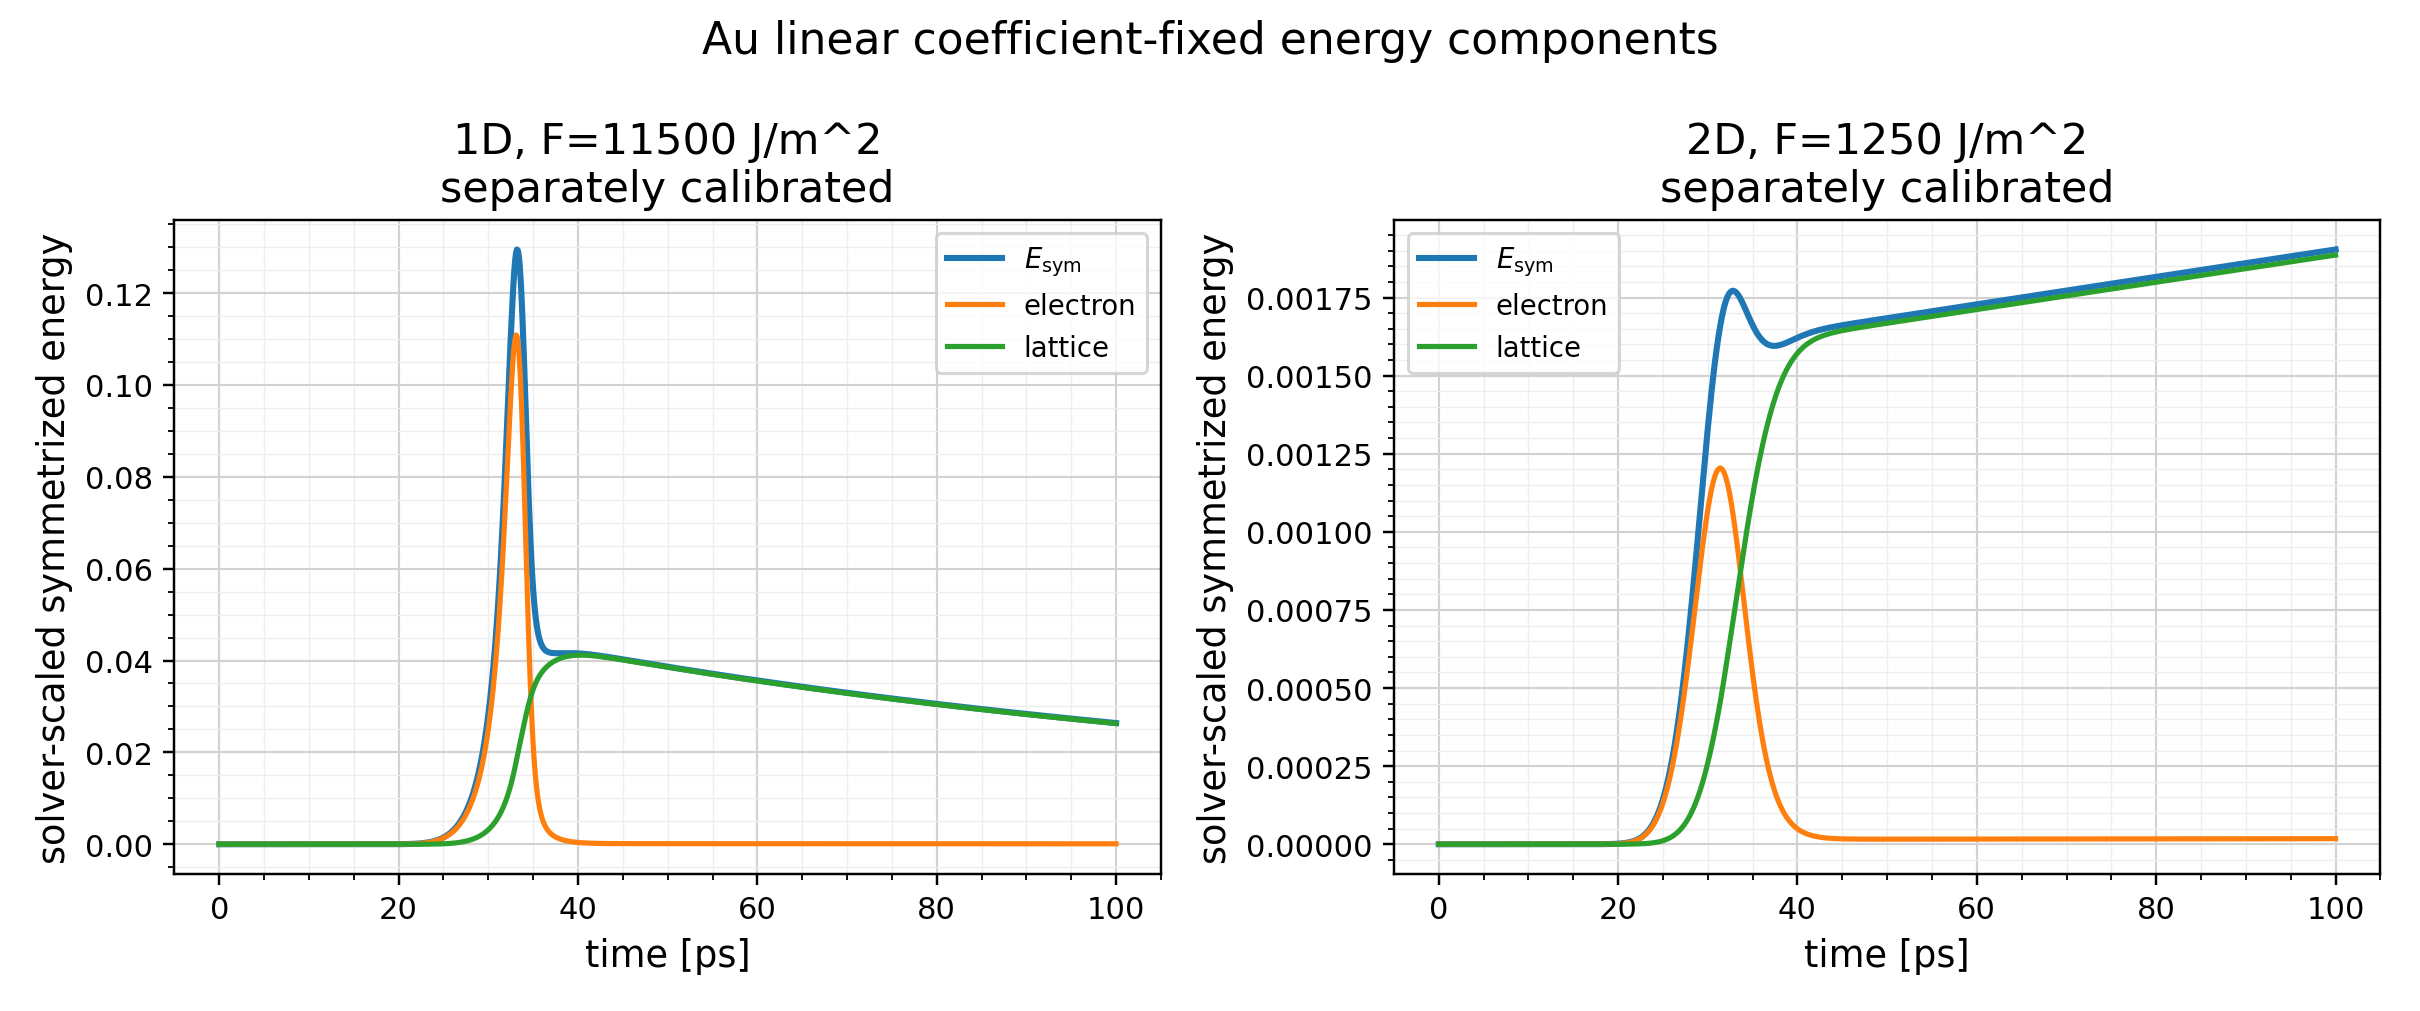
\includegraphics[width=0.95\textwidth]{figures/ch2/energy_diagnostics/thesis_energy_components_1d_2d.png}
    \caption{Solver-scaled symmetrised energy components for linear Au pTTM diagnostics in 1D and 2D. The fluence is calibrated separately in each dimension to remain sub-threshold while producing an informative accepted-slice diagnostic.}
    \label{fig:app-ch2-energy-components-diagnostics}
\end{figure}

\begin{figure}[htbp]
    \centering
    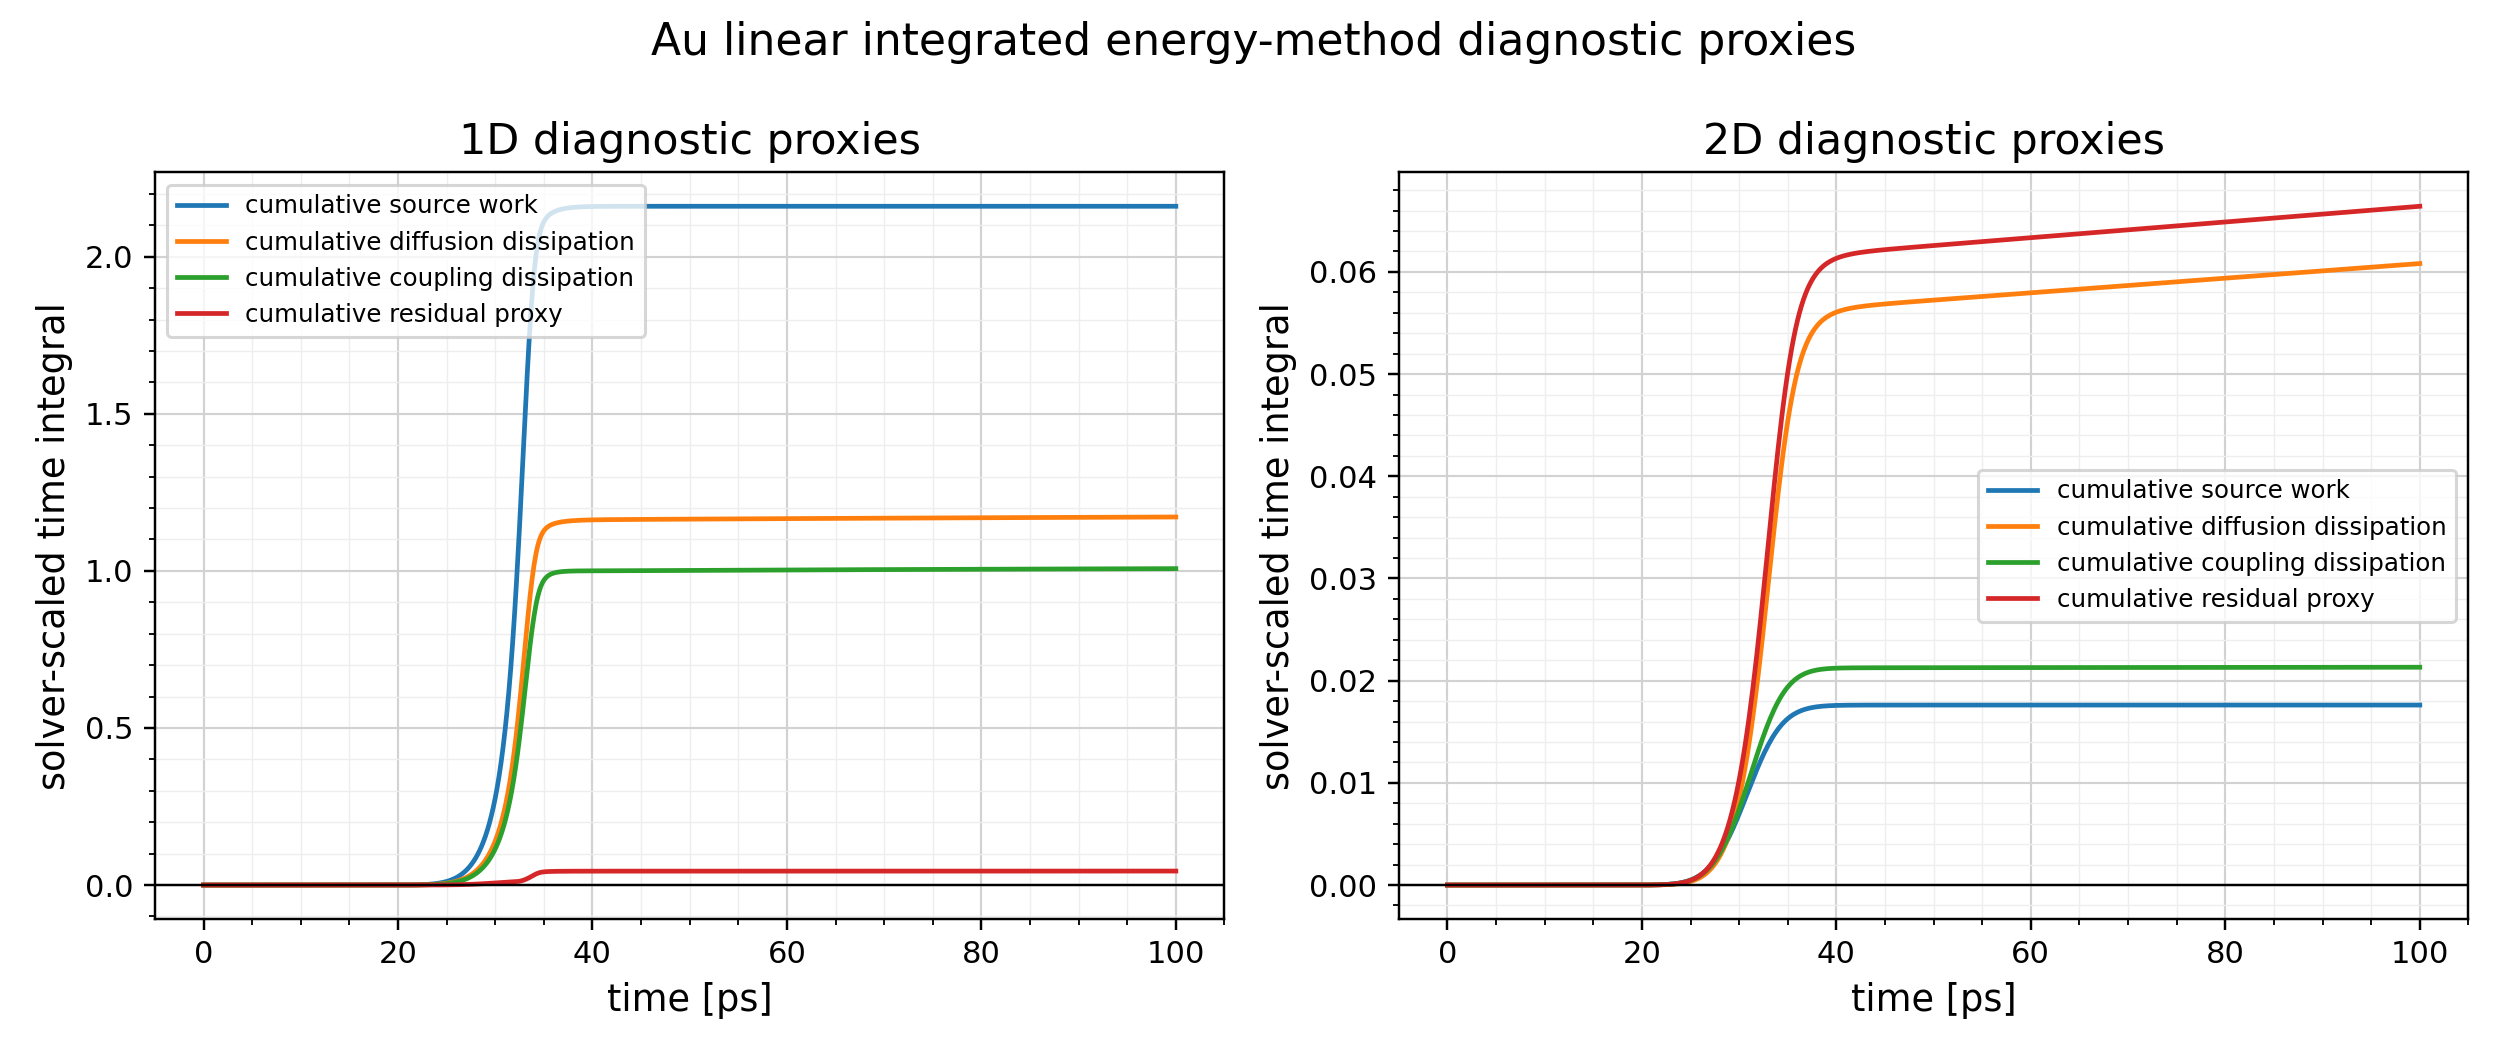
\includegraphics[width=0.95\textwidth]{figures/ch2/energy_diagnostics/thesis_integrated_terms_1d_2d.png}
    \caption{Cumulative source, diffusion-dissipation, coupling-dissipation, and residual proxies for the linear Au 1D and 2D diagnostics.}
    \label{fig:app-ch2-integrated-terms-diagnostics}
\end{figure}

The energy-component plot shows bounded symmetrised energy traces for both benchmark dimensions. The integrated-term plot shows the accepted source input competing with diffusion and coupling dissipation proxies, while the residual proxy measures finite-difference and source-reconstruction mismatch. The nonlinear pTTM is not assessed here because Appendix~\ref{app:ch2-rectangular-energy} proves only the coefficient-fixed rectangular estimate.
